\section*{Dati e risultati}

\subsection*{Slew Rate}

Per iniziare cerchiamo di capire cosa sia lo Slew Rate. In elettronica lo Slew Rate ($SR$) è definito come la massima variazione di tensione in uscita ($V\ped{out}$) per unità di tempo, quindi in formle abbiamo:
\begin{equation}
	SR\,=\,\frac{\Delta V}{\Delta t}
	\label{slew_rate_equation}
\end{equation}
dove con $\Delta V$ abbiamo indicato la differenza di potenziale in uscita dal circuito e con $\Delta t$ l'intervallo temporale preso in esame.
Pertanto questo fattore indica la velocità di risposta di un dispositivo o circuito elettronico ad una rapida variazione di tesione in ingresso in un intervallo di tempo molto piccolo. Queste variazioni di tensione darebbero luogo a segnali che in uscita varierebbero troppo rapidamente per poter essere riprodotte dallo strumento. Infatti ogni apparato fisico è in grado di erogare quantità di correnti limitate e non infinite, pertanto si possono generare differenze di potenziale che non eccedono questa quantità ovvero la velocità di risposta o Slew Rate.

Quindi per misurare effettivamente lo Slew Rate abbiamo realizzato il circuito riportato in Figura \ref{fig:slew_rate}. Le caratteristiche di questo circuito sono le seguenti: la tensione di alimentazione positiva ($V\ped{cc}^+$) vale $\SI{+15}{\volt}$ mentre quella negativa ($V\ped{cc}^-$) vale $\SI{-15}{\volt}$. All'ingresso non invertente ($V_p^+$) abbiamo deciso di fornire come segnale in entrata un'onda quadra in quanto, a nostro parere, è il tipo di imput più adatto per studiare questo fenomeno. Il segnale in ingresso ha le seguenti caratteristiche: frequenza ($\nu$) di $\SI{1}{\kilo\hertz}$ e differenza di potenziale picco-picco di $\SI{10}{\volt}$. Il circuito collegato all'uscita dell'OPAMP è stato realizzato su suggrimento del costruttore e il valore di resistenza usato vale $R\,=\,\SI{2.2}{\kilo\ohm}$, mentre per la capacità abbiamo usato un capacitore da $C\,=\,\SI{180}{\pico\farad}$.

Tuttavia prima di andare a ricavare il valore dello Slew Rate del nostro circuito abbiamo deciso di valutare quello del nostro generatore di forme d'onda. Un valore approssimativo, probabilmente stimato in eccesso è: $SR\ped{0}\,=\,0.5\,\frac{\SI{}{\volt}}{\SI{}{\nano\second}}$.

A questo punto, grazie all'oscilloscopio, siamo andati ad acquisire le forme d'onda del segnale in ingresso e in uscita dal nostro circuito. Quindi andando ad analizzare i dati ottenuti, riportati in Figura \ref{fig:slew_rate_plot}, abbiamo ottenuto che, per il nosro amplificatore operazionale $UA741$, gli Slew Rate di salita e discesa  valgono:
\begin{equation}
	SR_s\,=\,\frac{90\%V\ped{out}-10\%V\ped{out}}{t\ped{90\%}-t\ped{10\%}}\,=\,(0.498\,\pm\,0.004)\,\frac{\SI{}{\volt}}{\SI{}{\micro\second}}
	\label{slew_rate_value_s}
\end{equation}
\begin{equation}
	SR_d\,=\,\frac{90\%V\ped{out}-10\%V\ped{out}}{t\ped{90\%}-t\ped{10\%}}\,=\,(-0.353\,\pm\,0.003)\,\frac{\SI{}{\volt}}{\SI{}{\micro\second}}
	\label{slew_rate_value_d}
\end{equation}
dove con $SR_s$ indichiamo lo Slow Rate del fronte d'onda in salita, mentre $SR_d$ è relativo al fronte d'onda in discesa.
Come è possibile notare vi sono ben tre ordini di grandezza tra lo Slew Rate del generatore di forme d'oda e quelli del nostro amplificatore. Per questo motivo possimo considerare ininfluente il cotributo al ritardo del segnale dovuto al generatore di forme d'onda.

Inoltre nei grafici in Figura \ref{fig:slew_rate_plot} sono illustrati due esempi del fenomeno sopra anlizzato.

%\begin{figure}[]
%        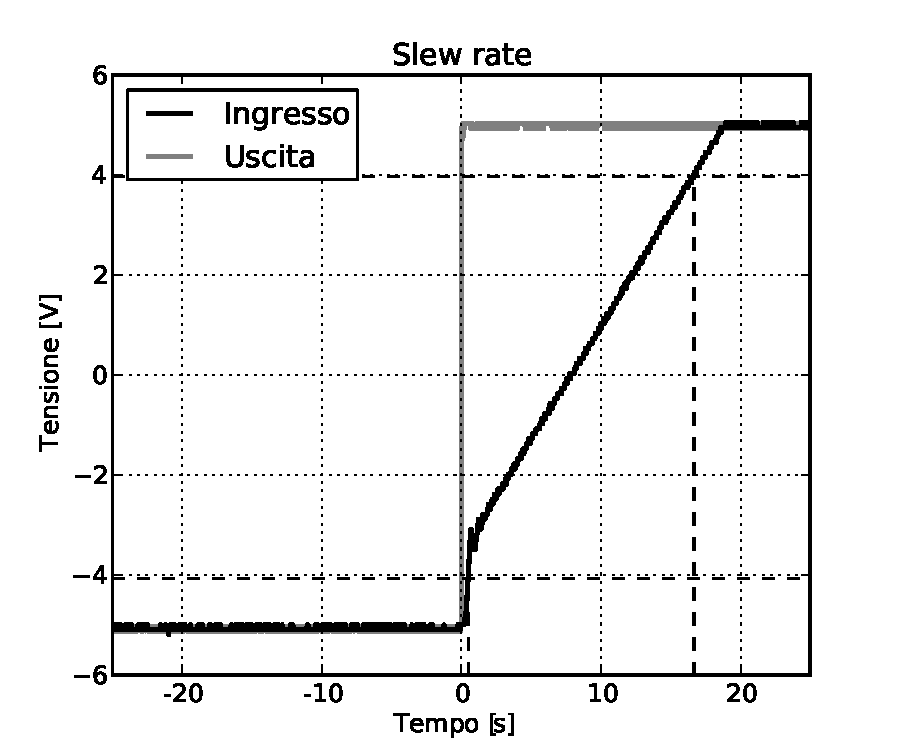
\includegraphics[scale=0.5]{Figure/slew_graph1.pdf}
%        \caption{La figura mostra il comportamento dell'amplificatore operazionale ad un brusco cambiamento della tensione differenziale in ingresso. Il circuito realizzato (Figura \ref{fig:slew_rate}) è un emitter follower e dovrebbe copiare il segnale in ingresso all'uscita. Invece, a causa del fatto che lo slew rate dell'operazionale è finito, la tensione impiega circa 20 $\mu$s a passare da -5 V a 5 V.}
%        \label{fig:slew_rate_plot1}
%\end{figure}

%\begin{figure}[]
%        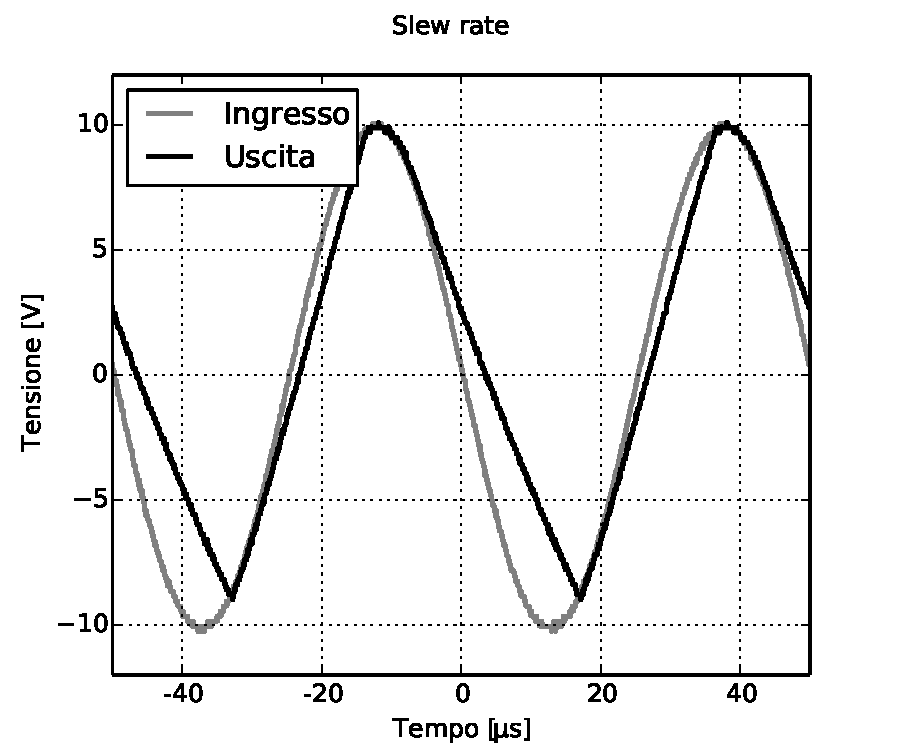
\includegraphics[scale=0.5]{Figure/slew_signal3.pdf}
%        \caption{La figura mostra il comportamento dell'amplificatore operazionale ad un brusco cambiamento della tensione differenziale in ingresso. Il circuito realizzato (Figura \ref{fig:slew_rate}) è un emitter follower e dovrebbe copiare il segnale in ingresso all'uscita. Invece, a causa del fatto che lo slew rate dell'operazionale è finito, la tensione impiega circa 20 $\mu$s a passare da -5 V a 5 V.}
 %       \label{fig:slew_rate_plot2}
%\end{figure}

\subsection*{Corrente massima erogabile}

In questo paragrafo vogliamo invece valutare la corrente massima ($I$) erogabile dal nostro amplificatore operazionale. Per farlo abbiamo sfruttato il circuito riportato in Figura \ref{fig:current}

Le caratteristiche di questo circuito sono le seguenti: la tensione di alimentazione positiva ($V\ped{cc}^+$) vale $\SI{+15}{\volt}$ mentre quella negativa ($V\ped{cc}^-$) vale $\SI{-15}{\volt}$. Come segnale di input all'ingresso non invertente ($V_p^+$) abbiamo deciso di usare una forma d'onda a dente di sega di frequenza ($\nu$) $\SI{500}{\hertz}$ e con una differenza di potenziale picco-picco di $\SI{10}{\volt}$. Il valore della resistenza di output vale $R\,=\,\SI{100}{\ohm}$.

L'idea che vogliamo seguire per misurare la corrente massima ($I\ped{max}$) erogabile dall'OPAMP e quella di creare un collegamento al comune dell'output mediante una resistenza molto piccola in modo che questa assorba quasi tutta la corrente erogata dall'amplificatore. In questo modo grazie all'oscilloscopio andremo a misurare la differenza di potenziale dell'output ($V\ped{out}$) e sfruttando la legge di Ohm è possibile ricavare il valore della corente ($I\ped{max}$), ovvero:
\begin{equation}
	I\ped{max}\,=\,\frac{\Delta V}{R}\,=\,(13.5\,\pm\,0.7)\,\SI{}{\milli\ampere}
\end{equation}

\subsection*{Banda passante dell'amplificatore operazionale}

In questo paragrafo vogliamo discutere del problema del guadagno dell'amplificatore oparazionale in funzione delle frequeanze dei segnali AC in entrata. A tal fine abbiamo realizzato il circuito in Figura \ref{fig:banda_passante}.

%\begin{SCfigure}
%	\def\svgwidth{0.5\textwidth}
%    \subimport{Figure/}{banda_circ.pdf_tex}
%    \caption{Circuito usato per misurare la banda passante dell'amplificatore operazionale.}
%    \label{fig:banda_passante}
%\end{SCfigure}

\begin{wrapfloat}{figure}{I}{0pt}
        \def\svgwidth{0.48\textwidth}
        \subimport{Figure/}{banda_circ.pdf_tex}
        \caption{Circuito usato per misurare la banda passante dell'amplificatore operazionale. E' un amplificatore operazionale usato in configurazione non invertente con circuito di retroazione negativa.}
        \label{fig:banda_passante}
\end{wrapfloat}

Le caratteristiche di questo circuito sono le seguenti: la tensione di alimentazione positiva ($V\ped{cc}^+$) vale $\SI{+15}{\volt}$ mentre quella negativa ($V\ped{cc}^-$) vale $\SI{-15}{\volt}$. Come segnale di input all'ingresso invertente ($V_p^-$) abbiamo deciso di usare una forma d'onda sinusoidale di frequenza ($\nu$) variabile e con una differenza di potenziale picco-picco di $\SI{50}{\milli\volt}$. I valori delle resistenze sono i seguenti: $R_1\,=\,\SI{10}{\kilo\ohm}\,/\,\SI{100}{\kilo\ohm}$ e $R_2\,=\,\SI{1}{\kilo\ohm}$. Facciamo notare che abbiamo deciso di applicare duna differenza di potenziale in ingresso così bassa per evitare problemi con lo Slew Rate del nostro amplificatore operazionale.

Per evitare che le misure acquisite siano alterate dalla tensione di offset abbiamo deciso di usare il trimer per azzerarla. Siamo riusciti ad avere una tensione di offset del valore di $V\ped{os}\,=\,\SI{5}{\milli\volt}$.

Come prima cosa abbiamo deciso di studiare come varia il guadagno del nostro circuito al variare della frequenza del segnale in ingresso nel caso in cui il circuito abbia un guadagno ($G$) di 10 o 20 decibell. Per fare questo abbiamo deciso di adottare i seguenti valori di resistenza: $R_1\,=\,\SI{10}{\kilo\ohm}$ e $R_2\,=\,\SI{1}{\kilo\ohm}$. In questo modo il rapporto tra $\frac{V\ped{out}}{V\ped{in}}\,=\,10$. A questo punto, grazie all'oscilloscopio, abbiamo acquisito i valori della tensione di output per vari valori di frequenza. Il risultato ottenuto è illustrato nel grafico in Figura \ref{fig:DB_plot}.
Abbiamo seguito una procedura analoga nel caso in cui il nostro circuito abbia un guadagno ($G$) di 100 o 40 decibell. Per fare questo abbiamo deciso di adottare i seguenti valori di resistenza: $R_1\,=\,\SI{100}{\kilo\ohm}$ e $R_2\,=\,\SI{1}{\kilo\ohm}$. In questo modo il rapporto tra $\frac{V\ped{out}}{V\ped{in}}\,=\,100$. Il risultato ottenuto è illustrato nel grafico in Figura \ref{fig:DB_plot}.

\begin{figure}[H]
    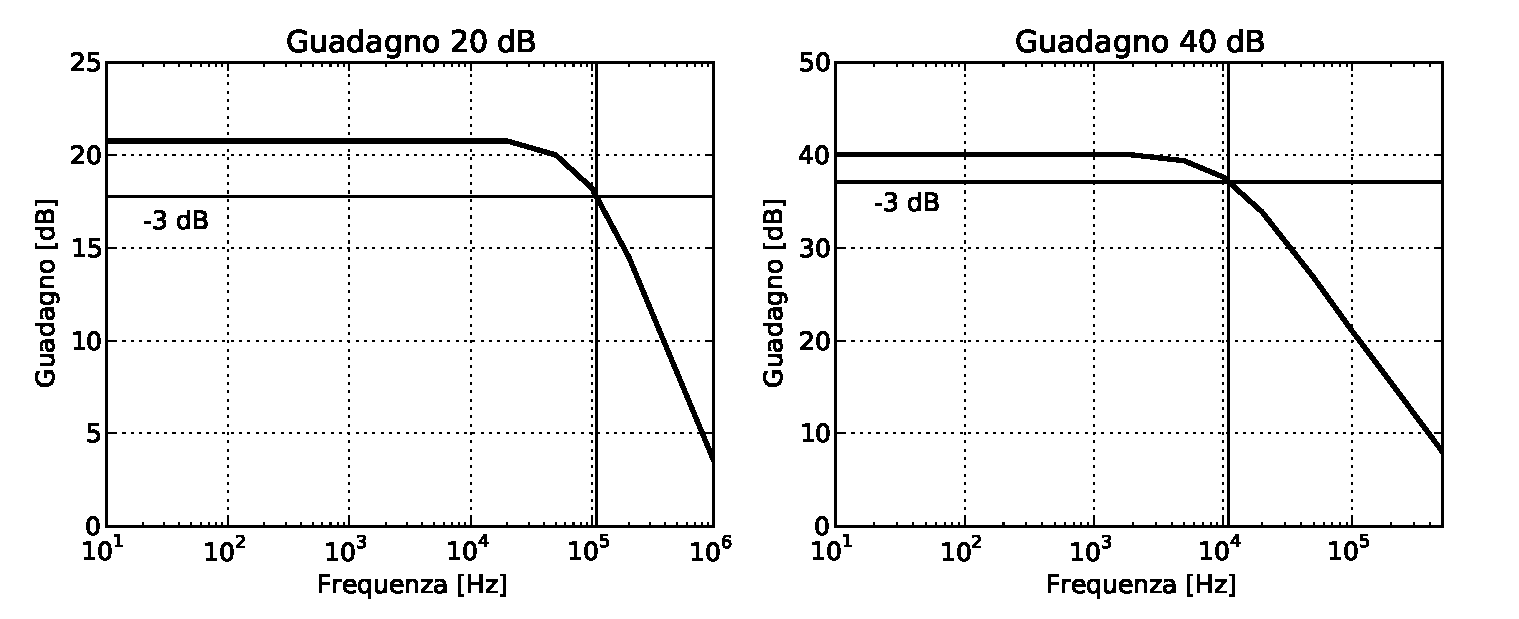
\includegraphics[width=\textwidth]{Figure/freq_ris.pdf}
    \caption{La figura mostra l'amplificazione in frequenza del circuito in Figura \ref{fig:banda_passante} nelle due varianti con guadagno di 20 db e 40 db circa. I circuiti si comportano come filtri passa basso con frequenza di taglio di $108 \pm 6$ kHz (20 db) e $11 \pm 5$ kHz (40 db). Sono filtri di primo ordine, con un'attenuazione di 20 db per decade.}
    \label{fig:DB_plot}
\end{figure}

Come si evince dai grafici riportati in Figura \ref{fig:DB_plot} si nota immediatamente che l'amplificatore operazionale non ha un comportamneto ideale in quanto il guadagno non è costante per tutti i valori di resistenza in ingresso. Infatti vi è un range di valori per i quali l'amplificazione rimane costante. Questo range è appunto la banda passante del nostro amplificatore operazionale. Abbiamo ottenuto infatti che:
\begin{itemize}\itemsep2pt \parskip0pt \parsep0pt
    \item{Banda passante per il circuito con gudagno di 20 dB: da zero a $108 \pm 6$ \SI{}{\kilo\hertz}.}
    \item{Banda passante per il circuito con gudagno di 40 dB: da zero a $11 \pm 5$ \SI{}{\kilo\hertz}.}
\end{itemize}
Inoltre è possibile notare come il circuito si comporti come un filtro passa basso. Infatti in entrambi i casi è possibile trovare il valore della frequenza di taglio ($\nu\ped{0}$) per cui il segnale in uscita è attenuato di 3 dB rispetto a quello di ingresso. In particolare abbiamo che:
\begin{itemize}\itemsep2pt \parskip0pt \parsep0pt
    \item{Circuito con guadagno di 20 dB: $\nu\ped{0}\,=\,(108\,\pm\,6)\SI{}{\kilo\hertz}$.}
    \item{Circuito con guadagno di 40 dB: $\nu\ped{0}\,=\,(11\,\pm\,5)\SI{}{\kilo\hertz}$.}
\end{itemize}

\subsection*{Guadagno open loop}

In quest'ultimo paragrafo ci proponiamo di studiare come varia il guadagno ($G$) del nostro amplificatore operazionale al variare della frequenza del segnale in ingresso ($V\ped{in}$) in configurazione circuitale open loop.

\begin{figure}[h]
        \centering
        \begin{subfigure}[b]{0.45\textwidth}
        	\def\svgwidth{\textwidth}
                \subimport{Figure/}{guad_freq_bassa_circ.pdf_tex}
                \caption{Circuito usato per misurare il guadagno $G$ del'amplificatore a basse frequenze. L'amlificatore operazionale è usato in configurazione invertente.}
                \label{fig:G_open_loop_basso}
        \end{subfigure}
        ~
        \begin{subfigure}[b]{0.45\textwidth}
        	\def\svgwidth{\textwidth}
                \subimport{Figure/}{guad_freq_alta_circ.pdf_tex}
                \caption{Circuito usato per misurare il guadagno $G$ del'amplificatore ad alte frequenze. L'amlificatore operazionale è usato in configurazione invertente.}
                \label{fig:G_open_loop_alto}
        \end{subfigure}
        \caption{}
\end{figure}

A tal fine abbiamo realizzato i circuiti riportati nelle Figure \ref{fig:G_open_loop_basso} e \ref{fig:G_open_loop_alto}. Le caratteristiche di questi circuiti sono le seguenti: la tensione di alimentazione positiva ($V\ped{cc}^+$) vale $\SI{+15}{\volt}$ mentre quella negativa ($V\ped{cc}^-$) vale $\SI{-15}{\volt}$. Come segnale di input all'ingresso invertente ($V_p^-$) abbiamo deciso di usare una forma d'onda sinusoidale di frequenza ($\nu$) variabile e con una differenza di potenziale picco-picco di $\SI{50}{\milli\volt}$. Abbiamo scelto questo valore sempre per evitare problemi con lo Slew Rate dell'amplificatore operazionale.

Il primo circuito, in Figura \ref{fig:G_open_loop_basso}, è stato usato per misurare il guadagno $G$ dell'amplificatore operazionale per frequenze inferiori alle centinaia di $\SI{}{\kilo\hertz}$. Abbiamo adottato questa particolare configurazione circuitale per il seguente motivo. Come osservato nel paragrafo precedente il guadagno dell'amplificatore operazionale è massimo per frequenze comprese tra i 10 e i 100  $\SI{}{\kilo\hertz}$. Pertanto un segnale in ingresso molto piccolo $\SI{50}{\milli\volt}$ viene amplificato notevolmente. Questo è dovuto anche al corretto funzionamento della retroazione negativa. Ora, proprio a causa della retroazione negativa, se facessimo una misura diretta della tensione ai capi dell'ingresso invertente $V^-$ otterremmo un valore di tensione troppo piccolo per essere letto correttamente dall'oscilloscopio, in quanto non ha una sufficiente sensibilità. Per questo motivo, usando la configurazione circuitale in Figura \ref{fig:G_open_loop_basso}, siamo in grado di ottenere il valore della tensione di $V^-$ in modo indiretto, sfruttando la differenza di potenziale $V_A$. Infatti vale che:
\begin{equation*}
        V^-\,=\,V_A\,\frac{R_4}{R_3+R_4}
\end{equation*}
e noi siamo in grado di misurare senza problemi la tensione in $V_A$. Pertanto dal momento che $V^+\,=\,\SI{0}{\volt}$ il nostro segnale in ingresso $V\ped{in}\,\equiv\,V^-$.
Il secondo circuito, in Figura \ref{fig:G_open_loop_alto}, è stato usato per misurare il guadagno $G$ dell'amplificatore operazionale per frequenze superiori alle centinaia di $\SI{}{\kilo\hertz}$. A queste frequene non abbiamo riscontrato problemi nella misura diretta della dfferenza di ptenziale in $V^-$, pertanto non ci sono ulteriori considerazioni da fare.

I risultati ottenuti sono riportati in Figura \ref{fig:G_openloop_plot1} e \ref{fig:G_openloop_plot2}

\begin{SCfigure}
    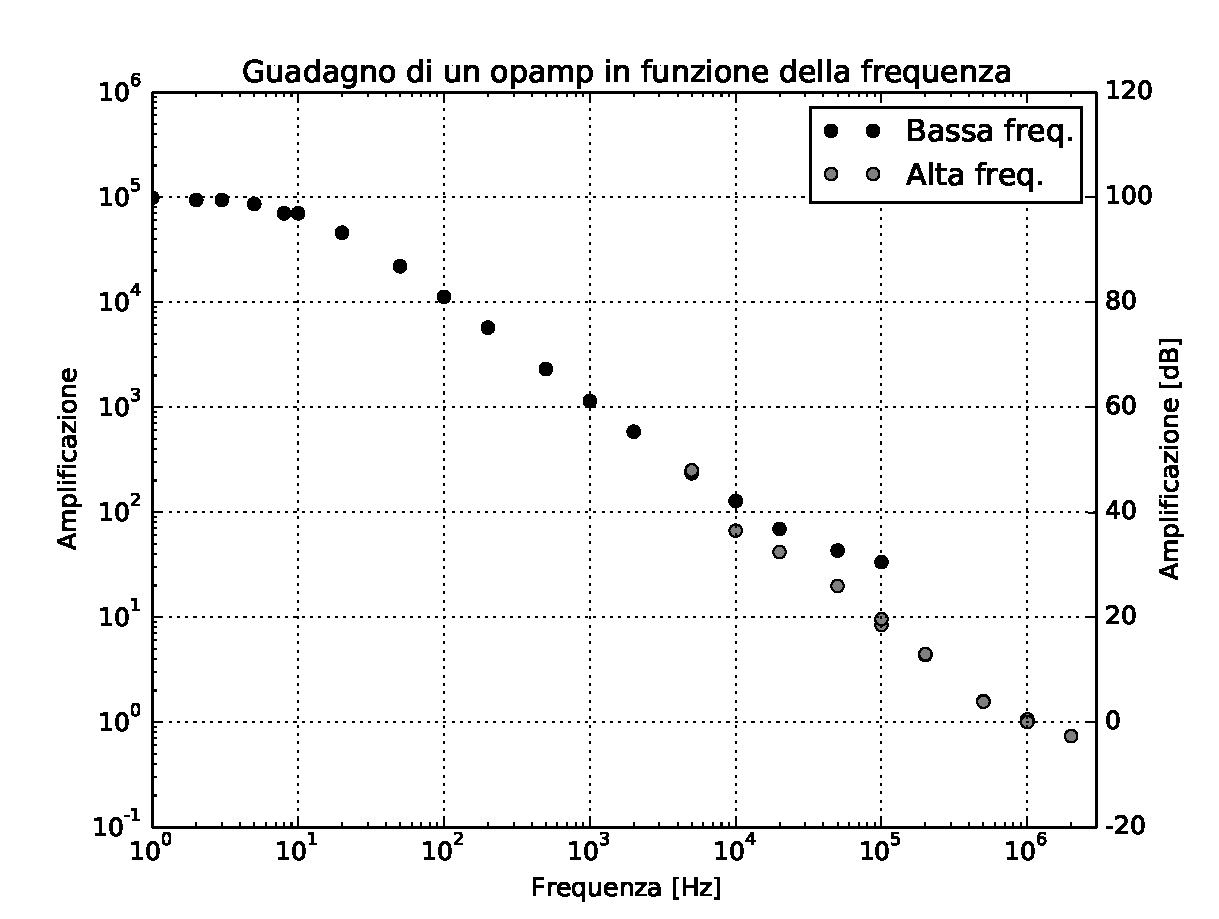
\includegraphics[width=0.7\textwidth]{Figure/A_vs_freq.pdf}
    \caption{Il grafico mostra l'andamento del guadagno open loop dell'amplificatore operazionale UA741 in funzione della frequenza. Come si vede il guadagno è massimo solo in una ristretta banda di frequenze, fino a circa 8 Hz. Poi il guadagno diminuisce ad un decimo ogni decade. I punti neri sono stati rilevati con il circuito \ref{fig:G_open_loop_basso} e si vede che a frequenze alte l'incertezza diventa cospicua, mentre quelli grigi sono stati misurati con il circuito \ref{fig:G_open_loop_alto}. Nei punti dove l'incertezza non è visibile essa è minore della dimensione dei punti. Il guadagno diventa unitario a circa 1 MHz.}
    \label{fig:G_openloop_plot1}
\end{SCfigure}

\begin{SCfigure*}
    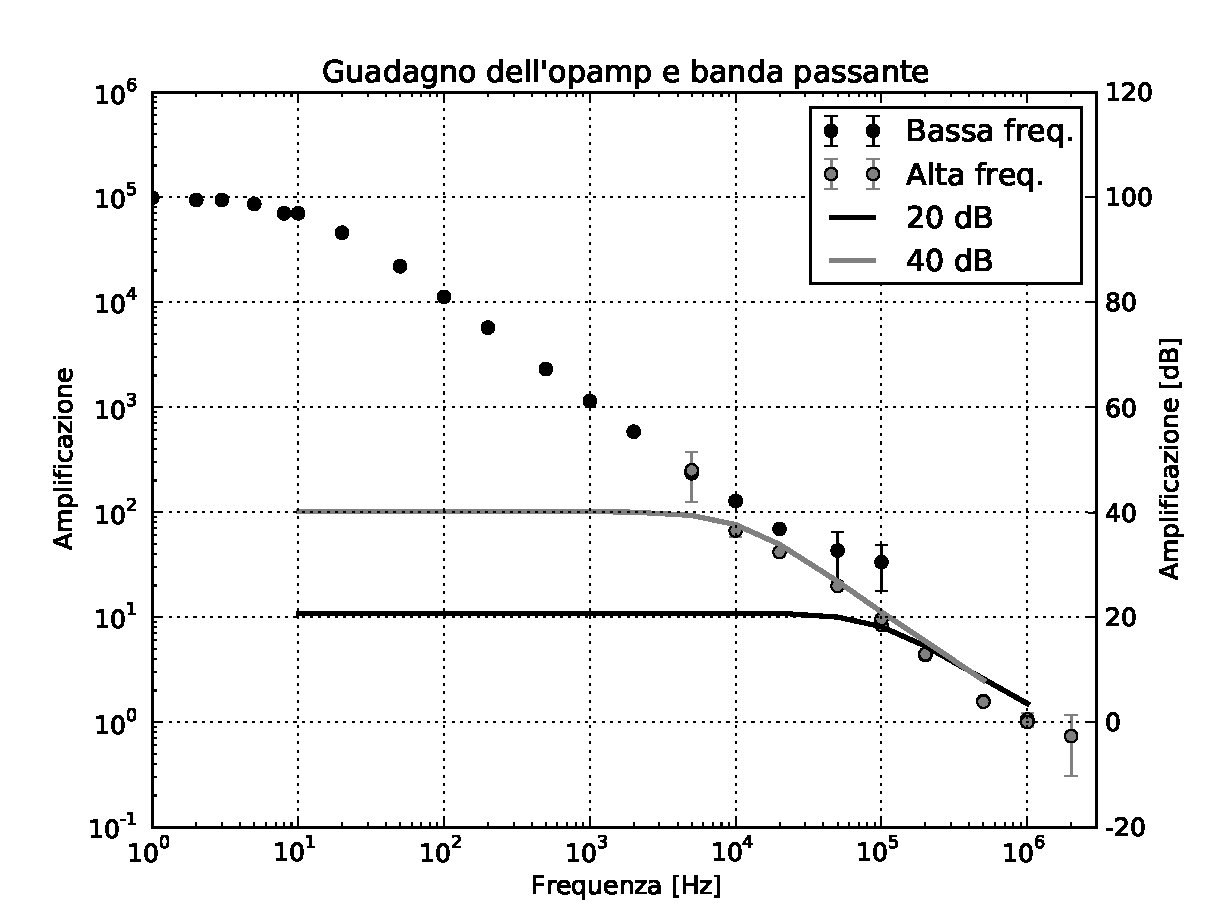
\includegraphics[width=0.7\textwidth]{Figure/gabp.pdf}
    \caption{Nel grafico sono visibili gli stessi dati delle Figure \ref{fig:DB_plot} e \ref{fig:G_openloop_plot1}. Come si può notare è proprio a causa dell'andamento del guadagno in funzione della frequenza dell'OPAMP che questi circuiti hanno una frequenza di taglio ed una riduzione del guadagno. Come riportato nella didascalia la linea grigia mostra l'andamento del guadagno del circuito (Figura \ref{fig:banda_passante}) con $G$ ideale di 20 dB, mentre la linea nera è relativa ad un guadagno ideale $G$ di 40 dB. Per la discussione sulle incertezze di misura si rimanda alla discussione fatta per il grafico in Figura \ref{fig:G_openloop_plot1}.}
    \label{fig:G_openloop_plot2}
\end{SCfigure*}
